\chapter{Methodology}

\section{Introduction}

The purpose of this chapter is to describe how the \ac{RAG} pipelines were built, tested, and assessed in this thesis. It will show how the theory on \acp{LLM}; semantic search, reranking, hybrid retrieval models, \ac{HPC} deployment, relate to the proposed experimental notebook-based workflow.

The methodology used a controlled comparative approach. First, a baseline RAG pipeline is created and subsequent pipeline versions are generated by adding different retrieval-levels. In order to allow for the attribution of differences in time, retrieval quality, and answer quality; mainly to the design choices made during retrieval and ranking, each version of the pipeline uses the same document set, query scenario sets, logging framework, and assessment process.

\section{Research Framework and Design}

The approach compares six \ac{RAG} pipeline variants. The implemented variants include a basic in-memory pipeline, a Milvus vector-database pipeline, a tuned vector-database pipeline, a reranking pipeline, a hybrid retrieval pipeline, and a hybrid retrieval with reranking pipeline. The main focus is to evaluate how these choices affect retrieval quality, answer quality, and execution time. The result logs identify these variants as \texttt{basic}, \texttt{vectordb}, \texttt{vectordb\_\allowbreak tuned}, \texttt{reranker}, \texttt{hybrid}, and \texttt{hybrid\_\allowbreak rerank}.

The comparisons were made by using a "local first" process. Each of the notebooks was initially tested on a local computer to evaluate the functionality of all code, services, prompts, results logging, and all evaluation script functions. The same workflow was executed in \ac{HPC} mode with changes to the model service and job execution to account for differences in environments. The only difference from the local environment in terms of how it executes was that the models were created on Slurm (an open source resource manager) and served as \ac{vLLM} (a cloud-based LLM model service), whereas the notebooks used the same pipeline structure and logging process.

By focusing on retrieving and ranking, and keeping the generator model consistent across experiments wherever possible, the comparison isolates the effects of changing retrieval components, including dense retrieval, persistent vector storage, tuned chunking, reranking, sparse-dense hybrid retrieval and hybrid retrieval with reranking.

\section{Dataset and Input Documents}
The experiments use the OrchestrAI synthetic enterprise dataset developed specifically for this project in a local project directory. This dataset includes 54 \texttt{.docx} files, which are located within ten different departmental folders (Customer Support, Engineering, Finance, Human Resources/HR, Information Technology /IT, Logistics, Product, Sales, Security and Q\&A Handbooks). In total the documents contain company policy and descriptions of policies; customer service procedures; on-boarding work flow; procurement processes; product development descriptions; as well as cross functional operational descriptions.

Each notebook uses the Haystack \texttt{DOCXTo\allowbreak Document} converter to load the same document set recursively. While documents are loaded, they are enriched with additional metadata – primarily the original source filename and department. This metadata is used in manually evaluating retrieved documents when the retrieved documents are saved to the \texttt{results.csv} for later comparison purposes. 

The different chunking configurations are unique to the chunking being used as a part of the experimental design. The baseline in memory pipeline has a chunk size of 120 words and an overlap of 20 words. The dense milvus, rerank, hybrid and hybrid rerank pipelines have a chunk size of 80 words and an overlap of 20 words. The vector database tuned pipeline has a much larger chunk size at 200 words, but also includes a larger overlap of 40 words. The remainder of the vector database configuration was kept constant in the tuned version such that the effect of chunk size could be evaluated more specifically.

\section{System Architecture}

The developed system follows the common \ac{RAG} architecture illustrated in Figure~\ref{fig:methodology-rag-architecture}. A user query is used to retrieve relevant document fragments. These fragments are then inserted into a prompt and provided to the \ac{LLM} as context. The model then, generates an answer based on the retrieved context and the original question.

\begin{figure}[htbp]
    \centering
    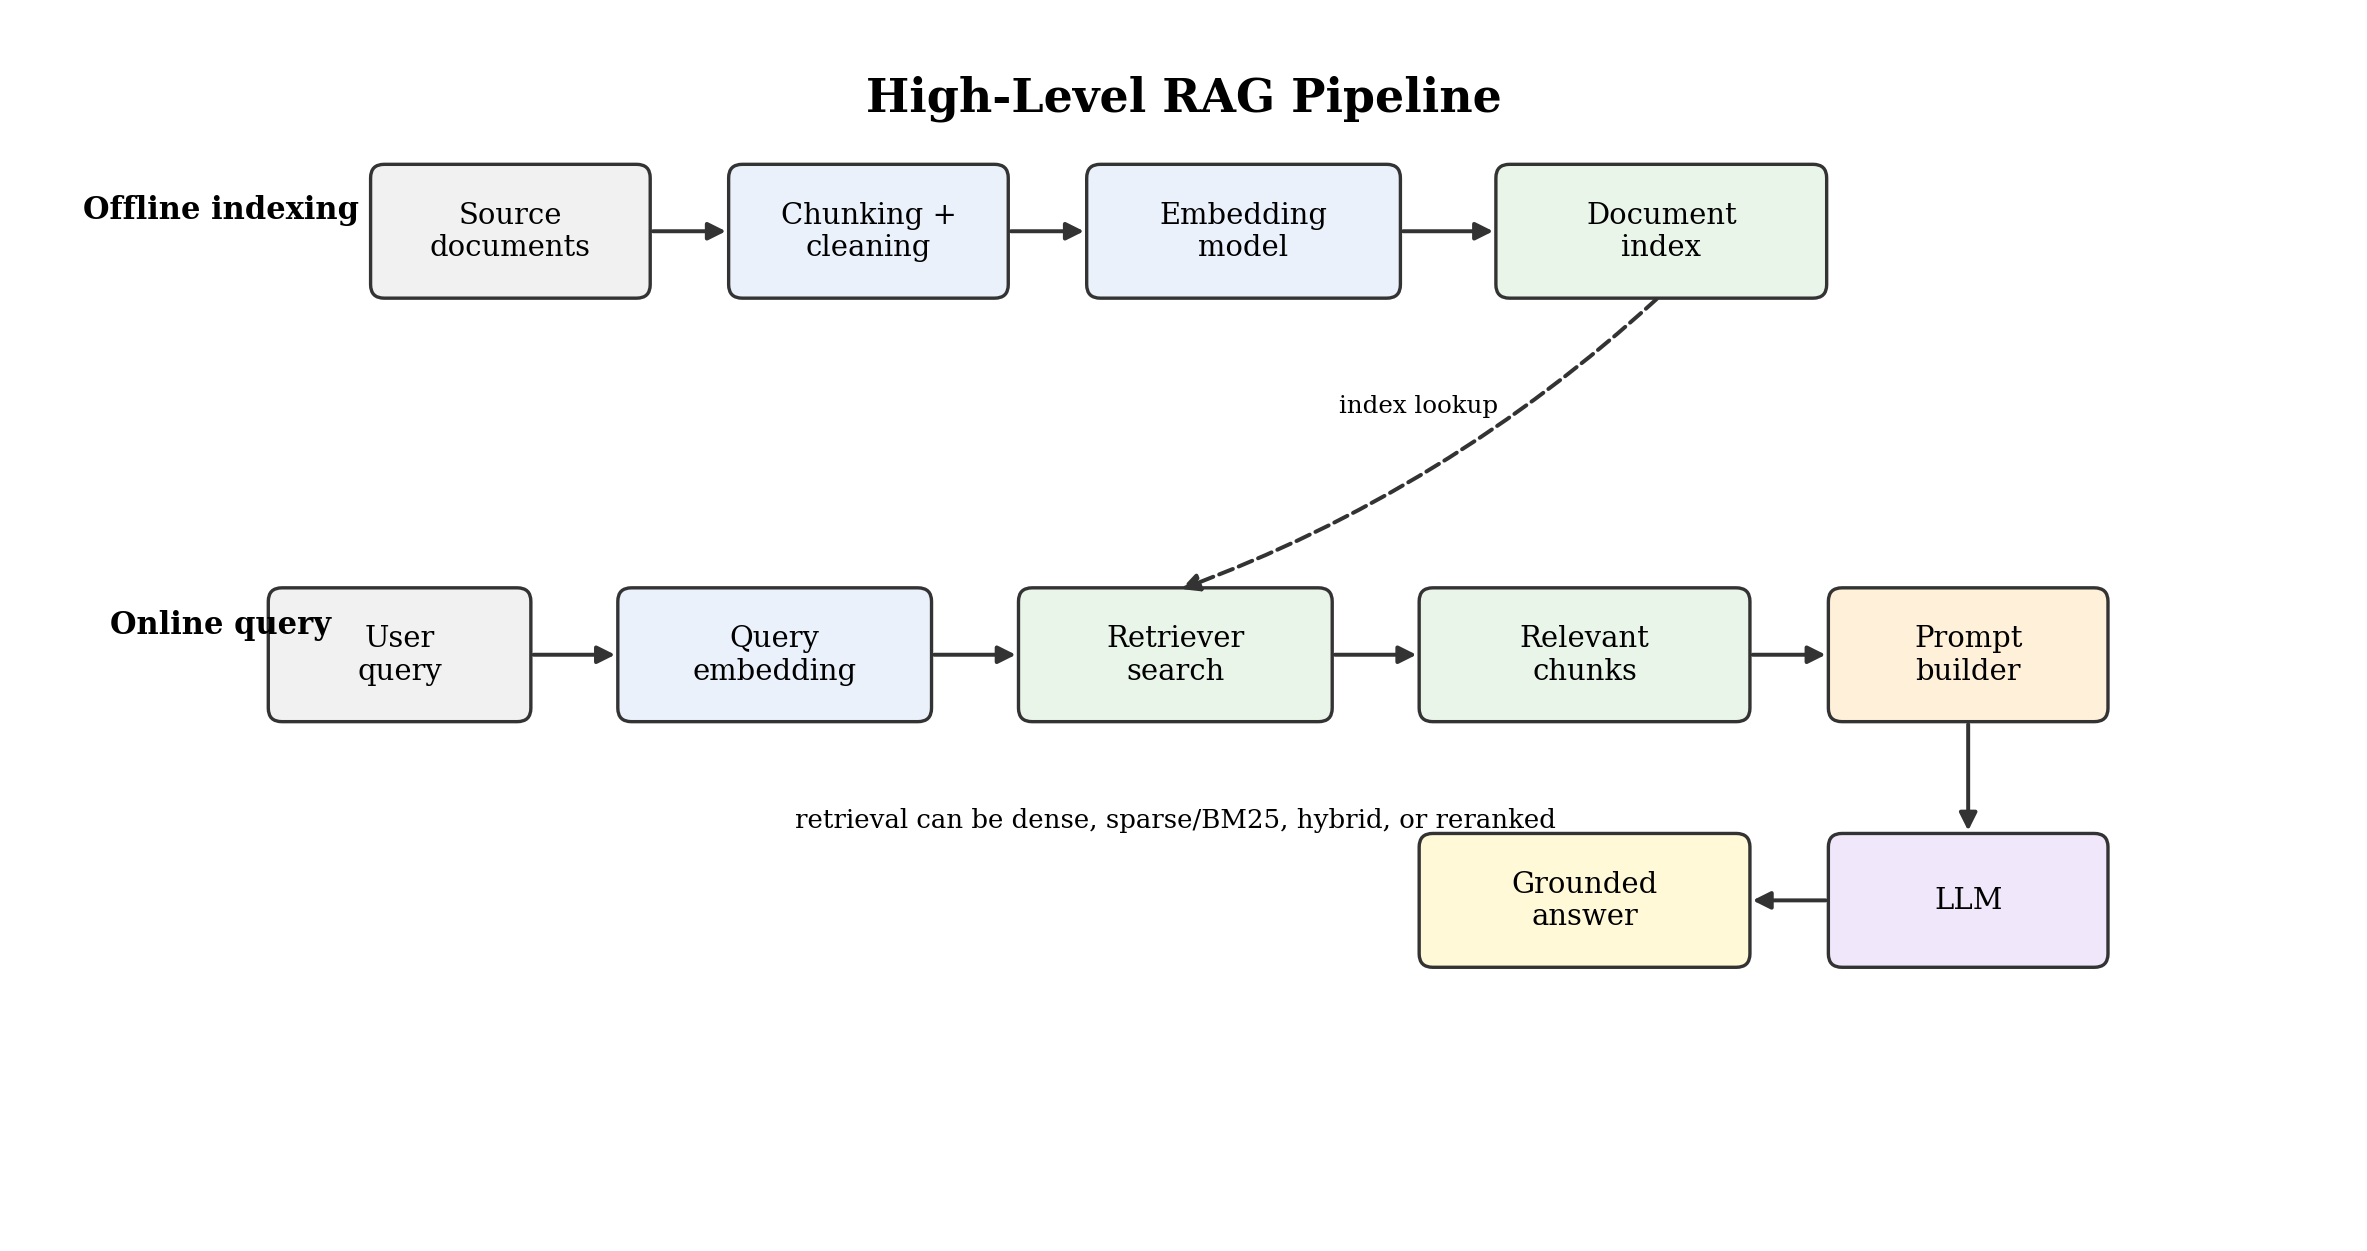
\includegraphics[width=\textwidth]{images/fig03_high_level_rag_pipeline.png}
    \caption{High-level RAG workflow used by the implemented notebooks: user query, retrieval over indexed documents, context construction, and answer generation.}
    \label{fig:methodology-rag-architecture}
\end{figure}

Haystack components are used in this application as document conversion, document spliting, document embedding, document retrieval, generating prompts and orchestrating generation workflows. When using a local workflow, Ollama will serve both the answer generation model (\texttt{llama3.1:8b}) and the embedding model (\texttt{mxbai-embed-large}). The milvus based version will access a local milvus instance that is being run by a shell script named \texttt{scripts/embed.sh}. A mini-lm cross encoder was used for local reranking of search results. This encoder was trained on \texttt{MS MARCO} ranking data.

The main architectural components are:

\begin{itemize}
    \item \textbf{Document loader and chunker:} Loads \texttt{.docx} files, stores source metadata, and splits documents into retrieval units.
    \item \textbf{Embedding model:} Converts each document chunk and user question into a dense vector representation.
    \item \textbf{Document store:} Stores chunks either in-memory or in Milvus, depending on the pipeline variant.
    \item \textbf{Retriever:} Uses dense vector similarity, sparse lexical retrieval, or hybrid sparse-dense retrieval to identify candidate chunks.
    \item \textbf{Reranker:} Reorders retrieved candidate chunks in the reranking variants before the final context is passed to the prompt builder.
    \item \textbf{Prompt builder and generator:} Combines the retrieved context with the user question and sends the question-context pair to the language model.
    \item \textbf{Results logger:} Writes the implementation name, scenario identifier, retrieved sources, generated answer, and timing values to a shared CSV file.
\end{itemize}

This structure supports fair comparison because all notebooks use the same high-level workflow while differing at the retrieval or ranking strategy level. It also supports \ac{HPC} execution because the notebooks and helper scripts can be executed in a managed environment with environment-specific setup changes.

\section{Implemented RAG Pipelines}

\begin{table}[htbp]
\centering
{\footnotesize X indicates that the component or configuration is part of the pipeline variant.\par}
\vspace{0.5em}
\scriptsize
\begin{tabularx}
{\textwidth}{>{\raggedright\arraybackslash}p{0.16\textwidth}*{8}{>{\centering\arraybackslash}X}}
\toprule
\textbf{Pipeline} & \textbf{In-memory docs} & \textbf{Vector DB} & \textbf{Dense retrieval} & \textbf{Sparse / BM25} & \textbf{Reranker} & \textbf{Tuned chunks} & \textbf{LLM generation} & \textbf{CSV logging} \\
\midrule
\texttt{basic} & X & - & X & - & - & - & X & X \\
\texttt{vectordb} & - & X & X & - & - & - & X & X \\
\texttt{vectordb\_\allowbreak tuned} & - & X & X & - & - & X & X & X \\
\texttt{reranker} & - & X & X & - & X & - & X & X \\
\texttt{hybrid} & - & X & X & X & - & - & X & X \\
\texttt{hybrid\_\allowbreak rerank} & - & X & X & X & X & - & X & X \\
\bottomrule
\end{tabularx}
\vspace{0.5em}
\caption{Implemented RAG pipeline variants and included components.}
\label{tab:six-rag-pipeline-variants}
\end{table}

\subsection{Baseline RAG version}
The baseline in-memory RAG version, \texttt{rag\_basic.ipynb}, utilizes an in-memory document store and an embedding-based retriever. The goal of this pipeline was to provide the simplest completely working \ac{RAG} model and serve as a reference point for the other versions. It demonstrated how retrieval and generation work when there is no added overhead of a vector database, sparse retrieval, or reranking.

\subsection{Version Using a Vector Database RAG}

The vector-database version, \texttt{rag\_vectordb.ipynb}, places document embeddings into Milvus. For each query, the version queries the Milvus collection and returns the top 10 dense matches. This version tested the effects of utilizing persistent vector databases as opposed to in-memory document stores.

\subsection{Tuned Version Using a Vector Database RAG}

The tuned vector-database version, \texttt{rag\_vectordb\_tuned.ipynb}, has the same Milvus backed dense retrieval structure as the standard vector-database pipeline. However, the primary differences were related to the chunking settings; specifically, the chunk size went up from 80 to 200 words while the chunk overlap increased from 20 to 40 words. This version evaluated whether larger chunks would provide more complete context to the generator and improve answer quality, while also testing the risk that larger chunks may reduce retrieval precision by mixing more content into each retrieved unit. Smaller chunks were not selected for this tuned version because the baseline Milvus configuration already used relatively short 80-word chunks.

\subsection{Reranking RAG}

The "reranking" version (\texttt{rag\_reranker.ipynb}) performs an initial search for 20 dense candidates with respect to the input using Milvus. It uses a cross encoder reranking model to reorder these candidates and selects the top 10 reranked candidates to be passed to the generator. As opposed to the vector database approach described in Section 4.5.2, this selection is made based on a larger candidate set (of size 20) that was previously generated as the result of an initial search. Therefore, it may help determine if a new relevance ordering step will sufficiently improve the quality of the contextual information provided by the system's previous output to warrant the added time delay for searching the database.

\subsection{Hybrid Retrieval RAG}

The hybrid version, \texttt{rag\_hybrid.ipynb}, used a hybrid retrieval mechanism made available by Milvus. It combines dense semantic embeddings, which support semantic matching, with a sparse BM25-style representation produced inside Milvus, which supports lexical matching. The goal of this version was to determine if semantic matching and lexical matching could be complementary. This is particularly interesting given that enterprise documents often contain exact term references (e.g., team name(s), severity level(s), product identifier(s), etc.).

\subsection{Hybrid Retrieval With Reranking RAG}

The hybrid-reranking version, \texttt{rag\_hybrid\_\&\_rerank.ipynb}, built upon the hybrid retrieval version. First, it retrieves 20 hybrid candidates. Next, it uses the cross-encoder reranker to select the top 10 documents for generation. This version may improve context ordering by combining dense retrieval, sparse lexical matching, and reranking, but it also increases retrieval cost: the time needed to perform the retrieval will increase since both hybrid candidate retrieval and reranking occur prior to the actual generation of answers.

\subsection{Measured Variables}

This thesis measures the following primary variables.

\begin{itemize} 
    \item Time to index in seconds
    \item Time to retrieve in seconds
    \item Time to generate in seconds
    \item Source files and departments that were retrieved
    \item Contexts that were retrieved
    \item Number of retrieved documents
    \item Top-k retriever and reranker values
    \item Generated answer text
    \item Correctness score and label given by manual assessment
    \item Deterministic measures of answer quality and retrieval quality. 
\end{itemize}

Most of the above-listed variables are logged to a common results log. These include the name of the used implementation, the id of the scenario, the question asked, the answer generated for this question, sources that were retrieved during the search process, departments that were retrieved during the search process, contexts that were retrieved during the search process, the number of documents that were retrieved from the database, the k-values for both retriever and reranker, time spent on indexing, time spent on retrieving information, and finally time spent generating answers. Additionally, manual correctness scores and labels for the answers can be added in an evaluation file provided with the ground truth.

The script for evaluating the answers deterministically will produce some additional quality metrics for the answers and for the retrieval. Time spent per query answering questions can be found in both the retrieval time and generation time. However, as indexing time does represent corpus preparation rather than question-answering latency directly, indexing time is reported separately. Finally, when comparing local vs. \ac{HPC} systems, the last line of the timing summary includes total runtime for each system's respective pipeline.

\section{Evaluation Framework}

\subsection{System Performance Metrics}

Both local and HPC run times for each experiment will be stored in the results csv file. In both cases, we use identical application-level timing fields (indexing time, retrieval time, generation time, and total execution time).

There are no new quality metrics introduced by \ac{HPC} evaluation. Instead, we compare the execution time of the same variant pipelines under a different execution environment. Although queue time, service startup time, and data transfer overhead may be important aspects of deploying your system, these were not considered to be separate experimental variables for this study.

\subsection{Retrieval Quality Metrics}

Retrieval quality is evaluated through comparison of the automatically retrieved source documents to the manual selection of supporting documents within the ground truth CSV. The proportion of manually selected supporting documents (out of all) that are retrieved is referred to as "recall". The ratio of manually selected supporting documents (out of all) to the total number of documents retrieved represents "precision." The retrieval F1 score is an average of both precision and recall. For each evaluation, we will be recording a "retrieval hit" if there exists at least one manually selected supporting document included in the automatically retrieved set.

\subsection{Answer Quality Metrics}

Manual evaluations assess the quality of the answer by providing a score to determine if the response was completely accurate, partially accurate, or completely inaccurate. Manual scoring assigns 1.0 for a fully correct answer, 0.5 for a partially correct answer, and 0.0 for an incorrect answer. 

The deterministic evaluation script computes additional automatically computed metrics. \ac{ROUGE-L} is a metric for measuring lexical overlap in addition to semantic similarity between the generated response and the reference response. \ac{BERTScore} is another metric that utilizes contextual embeddings to compute semantic similarities in addition to lexical overlap between the two responses. Similarly, a sentence transformer can measure the level of semantic similarity between individual sentences within each answer. Additionally, there are metrics related to the retrieval quality of the model such as whether enough supporting documents were retrieved. Lastly, the script will compute the average number of words in each generated answer.

\subsection{Visual Analysis}

Visualizations are produced via a visualization notebook that is specifically designed for visualizing results from which the final answers have been determined and processed. Timing breakdowns (per scenario), answer quality, retrieval quality and performance data per scenario will be shown. These figures are discussed in the results chapter 6 as part of an analysis on trade-offs among answer quality, retrieval quality, and execution time.

\subsection{Cross-Environment Comparison}

The local experiments are run with the notebook workflow with Ollama-based model serving and a local Milvus instance where needed. The \ac{HPC} experiments are run on the Cyclone \ac{HPC} \cite{cyi_cyclone} facility using Slurm-managed jobs and \ac{vLLM}-based model serving. Per the available info, Cyclone has CPU-only nodes and GPU-accelerated nodes, which have: \(2\times\) 20-core Intel Xeon Gold 6248 CPUs, \(4\times\) NVIDIA V100 accelerators, and 192 GB of memory per node.

The implemented \ac{HPC} workflow launches the model-serving components as separate Slurm jobs. \ac{LLM} generation service, embedding service, and reranking service each request one GPU and ten CPU cores. The \ac{LLM} service is \texttt{meta-llama/Llama-3.1-8B-Instruct}, the embedding service uses \texttt{BAAI/bge-m3} and the reranking service is \texttt{BAAI/bge-reranker-base}. These services expose connection information through environment files and are leveraged by the \ac{HPC} notebooks.

Although the six pipeline structures and timing variants are the same for the local and \ac{HPC} experiments, they are not identical model-serving deployments. The local workflow leverages the embedding with \texttt{mxbai-embed-large} and a local \ac{MiniLM} reranker. As such, the cross-environment comparison is more of a comparison of “workflow” level deployments and not an isolated hardware only benchmark.

The cross-environment comparison was for comparing application level timing behaviour, rather than attempting to evaluate any new retrieval logic, so the \ac{HPC} results are interpreted in the exact same way as the local results: indexing time, retrieval time, generation time, and total runtime.

\section{Reproducibility and Documentation}

Standardization of result collection is achieved through a logging system for all results. However, as already mentioned, the loggers will collect data for each notebook independent of other notebooks. Therefore, there are multiple \ac{RAG} pipelines being run with their own respective variants. All modules that are necessary for building ground truth and running the deterministic evaluation are separate from the notebooks. This allows to rerun the evaluation module at any time after the experimental data has been generated.

Documentation is necessary for reproducibility. Therefore, there is a \texttt{README} document for setting up the software and running each notebook, along with documenting how to start Milvus and what Ollama models are required, how to execute each notebook, what command to run to perform evaluation, where output files are written etc. The model serving scripts provide an additional layer of documentation of the workflow. In addition, Slurm submission commands and the location of the output CSV files are also documented. Lastly, code comments were added throughout the notebooks and helper scripts to explain why certain implementation steps were taken and what they accomplish.

\section{Summary}

The purpose of this chapter was to provide a detailed description of the methodologies that were employed to build out and evaluate the six \ac{RAG} pipeline variants as well as describe the common architectures and systems (dataset, pipeline variants, etc.) used to support testing and evaluation of these pipeline variants.

This chapter also provided an overview of the framework utilized to evaluate each of those pipeline variants with respect to timing, retrieval quality, answer quality, visual analysis, and the differences between local and \acf{HPC} environments.